\documentclass{article}
\usepackage{graphicx} % Required for inserting images
\usepackage{amsmath}
\usepackage{amssymb}
\usepackage{amsthm}
\usepackage{amsfonts}
\usepackage{gensymb}

\title{MathConstruction}

\begin{document}

\section{NCERT 12.10.5.9}

Find the position vector of a point R which divides the line joining two points P and Q whose Position Vectors are $2\vec{a}+\vec{b}$ and $\vec{a}-3\vec{b}$ externally in the ration $1:2$.Also, Show that P is the mid point of the line segment RQ \\
\textbf{Construction steps:}
\begin{enumerate}
    \item Let us consider vector of point R which divides the line joining two points P and Q externally in the ratio $m:n$ then for finding the external point R using section formulae.\\
    \begin{align}
        \Vec{OR}=\frac{n.\Vec{OP}-m.\Vec{OQ}}{n-m}
    \end{align}
    \item After finding point vector R we also know the point vectors P and Q,As given R is external point to find the mid point of line segment RQ we need to apply mid point formulae \\
    \begin{align}
        mid point =\frac{\Vec{OR}+\Vec{OQ}}{2}
    \end{align}
    if mid point vector is equal to the point vector P, then we can say that Point vector P is the mid point of the line segment RQ
    \item Let us, Assume Point vectors 
    \begin{align}
        \vec{OP}=2\vec{a}+\vec{b}\\
        \vec{OQ}=\vec{a}-3\vec{b}
    \end{align}
    and the ratio is 
    \begin{align}
        m:n=2:1
    \end{align}
    For finding the position vector R,
    \begin{align}
        \Vec{OR}=\frac{2(2\vec{a}+\vec{b})-1(\vec{a}-3\vec{b})}{2-1}\\
        \Vec{OR}=\frac{4\Vec{a}+2\Vec{b}-\Vec{a}+3\Vec{b}}{1}\\
        \Vec{OR}=3\Vec{a}+5\Vec{b}
    \end{align}
    \item Now The point vectors P,Q and R are
    \begin{align}
        \vec{OP}=2\vec{a}+\vec{b}\\
        \vec{OQ}=\vec{a}-3\vec{b}\\
        \Vec{OR}=3\Vec{a}+5\Vec{b}
    \end{align}
    For showing P is the midpoint of the line segment RQ
    \begin{align}
        \Vec{OP}=\frac{\Vec{OR}+\vec{OQ}}{2}\\
        \Vec{OP}=\frac{3\Vec{a}+5\Vec{b}+\vec{a}-3\Vec{b}}{2}\\
        \Vec{OP}=2\Vec{a}+\Vec{b}
    \end{align}
    So,it is proved that P is the midpoint of RQ.
    \item The Plot showing the Vector representation of the point vectors P,Q and R is
    \begin{figure}[!ht]
        \centering
        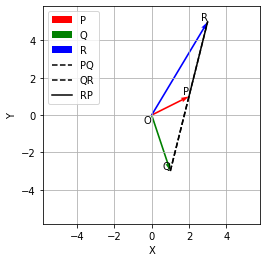
\includegraphics[width=\columnwidth]{/sdcard/geometry/math_computing/mathconstruction.png}
        \caption{point vectors P,Q,R}
        \label{fig:enter-label}
    \end{figure}
\end{enumerate}
\end{document}
